\section{Findings}
\label{cha:findings}


% Grading Criteria
% - Steps taken to arrive at the presented findings are clear 
%       => Das kann auch aus dem Background kommen, es muss nur klar sein wie die Ergebnisse zustande kommen
% - The research question is addressed
% - present findings
% - graphs and table support the main findings 
% - findings are presented without judgment

\section{How does the k-means Algorithm help to understand Electricity Load Patterns?}
\label{sec:findings_understand_electricity_load_patterns}
Conducting the literature review provided two different options for choosing the value of $k$ before executing k-means:
By choosing a fixed value the clustering results apply to criteria chosen in advance.
Liu et al \cite{LIU-BDE} choose a fixed value of $k=3$ since the clustering results are divided into low-, medium-, and high-consumption clusters.
By applying k-means with a variable value of $k$ the clustering results adapt to the data and therefore deliver problem-specific results.
Variable in this context means, that the value of $k$ is chosen problem-specific by using the elbow method.
This enables researchers to spot trends in the data without knowing about certain characteristics in advance.

Jessen et al. \cite{JES-IND} use k-means to analyze and label electricity load profiles of Lombok, Indonesia, as normal or abnormal.
The value for $k$ is chosen for each dataset specifically by using the elbow method.
Clustering the whole datasets of energy-load patterns in Lombok, Indonesia, resulted in Figure \ref{fig:whole_data_clustering_results}.
Each cluster holds approximately the data of a single year, for example, the black cluster contains data from 2015 and the red cluster contains mostly data from 2021.
This shows an overall increase in power consumption over the years.
The algorithm also managed to spot different consumption patterns in the data, with the lime cluster containing mostly the Ramadhan periods from 2018 to 2021.

To improve the overall understanding of the data, further theories and classifications can be applied after executing k-means.
The clustering results then fungate as input for higher-level models and theories.
This classification can take place by taking further datasets into account that underline the found characteristics and patterns.
Jessen et al. \cite{JES-IND} algorithmically label the clustering results into "normal" and "abnormal" clusters, with the abnormal clusters being natural disasters or electrical fault impacted.
This is done by comparing the clustering results with the occurrence time and epicenter of natural disasters and electrical faults.
By reapplying the clustering algorithm to the distinct clusters, the labeling process can be proven.
The clustering results for the earthquake-impacted year 2018 are shown in Figure \ref{fig:clustering_results_2018}.
Again, the algorithm divided the data into distinct clusters, with each cluster representing different consumption patterns.
Also, seasonal patterns are identified, since clusters containing mostly mid to low-consumption months like January and February or higher consumption months are spotted.
In this case, the algorithm managed to identify natural disaster-impacted clusters, as shown in the red cluster.
The red cluster contains post-natural disaster data, which is analyzed in greater detail in Figure \ref{fig:clustering_results_2018_cluster_two}.

These findings show, that k-means proves useful in understanding electricity load pattern datasets without prior knowledge.
By applying k-means, characteristics, patterns, and tendencies are spotted within the data.
The clustering results can be adjusted by choosing different values for $k$.
If a certain theory or defined categories want to be proven a fixed value is useful, to generate hidden knowledge out of large datasets a variable value is more useful.
This lays the groundwork for revealing hidden knowledge in the data, enabling more advanced methods to fully grasp the data's meaning.

\begin{figure}[H]
    \centering
    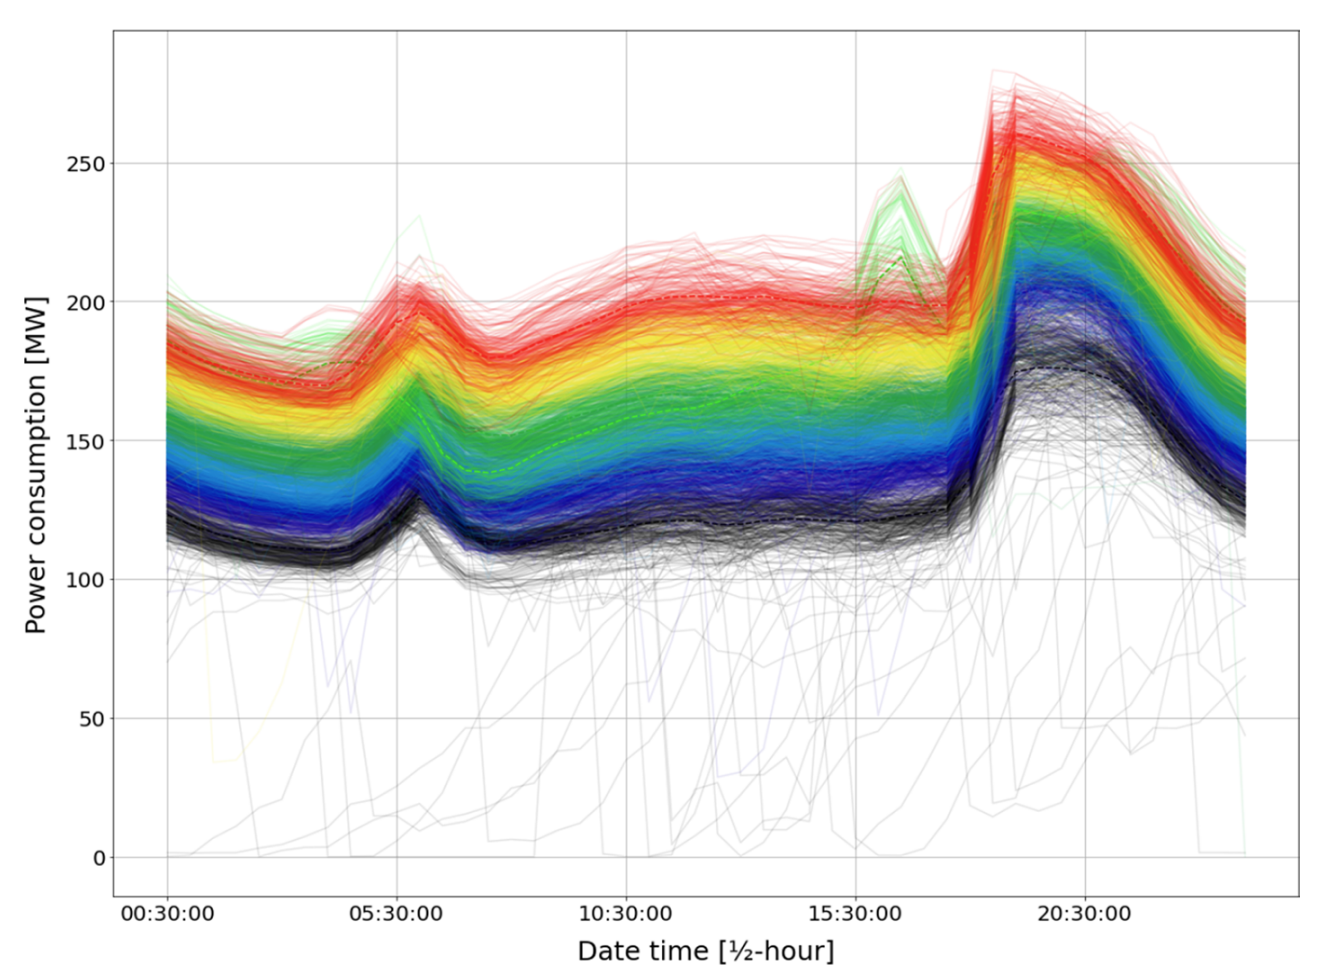
\includegraphics[width=0.6\textwidth]{figures/jessen_ndImpactedClusters/jessen_wholeDataClustering.png}
    \caption{These are the results of executing the k-means algorithm on the whole electricity load profile dataset of Lombok, Indonesia.
    The ideal number of clusters is proven to be $7$.
    Each cluster is represented by a different color.
    Each cluster approximately contains the electricity load profiles of one year.
    It is visible that the power consumption increased over the years since the clusters for the later years are more consuming than the clusters starting from 2015.
    Also, special events like the Ramadhan period are identified, here in the lime cluster.
    }
    \label{fig:whole_data_clustering_results}
\end{figure}

\begin{figure}[H]
    \centering
    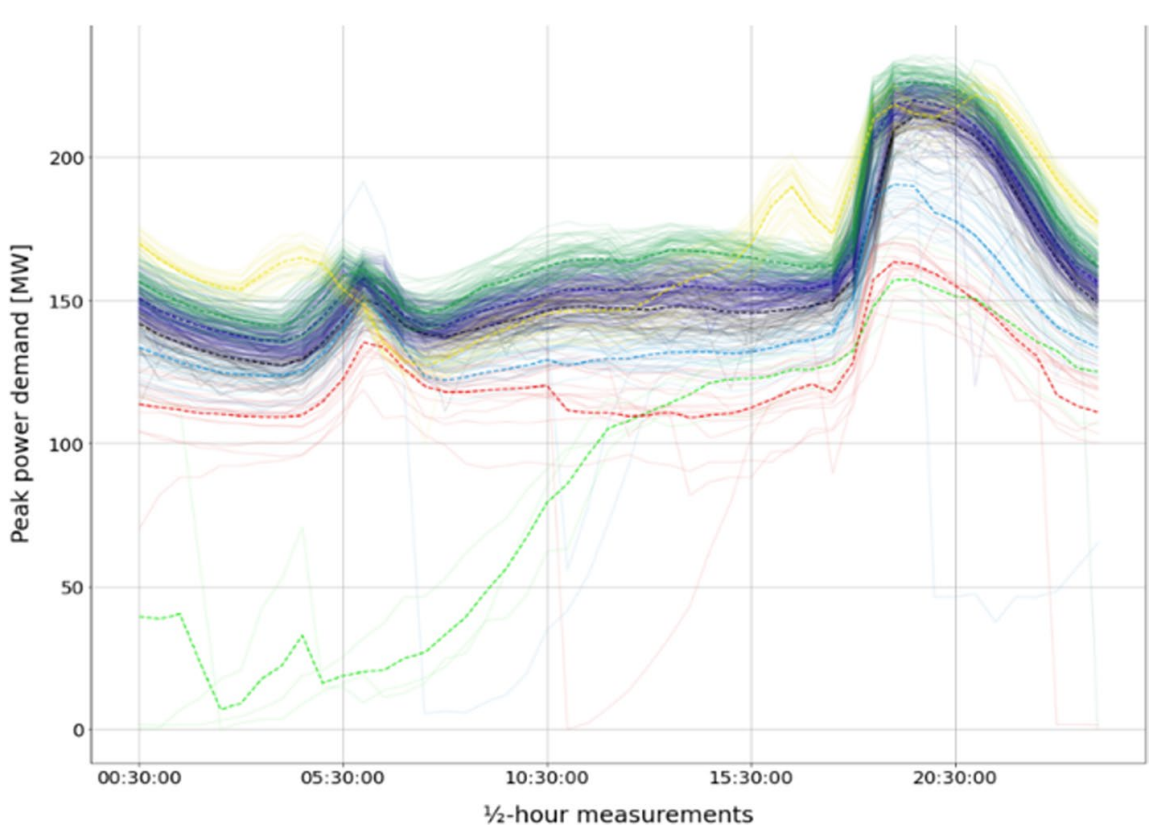
\includegraphics[width=0.6\textwidth]{figures/jessen_ndImpactedClusters/jessen_Clustering2018.png}
    \caption{This is the result of the k-means algorithm applied to the earthquake-impacted year of 2018.
    Again, the ideal number of clusters is proven to be $7$ with each cluster being represented by a different color.
    The clusters are divided into different consumption patterns showing different, non-earthquake-impacted consumption patterns.
    These patterns differ over the year.
    The black cluster contains mid to low-consumption months, mainly from January and February.
    Also, holiday periods like the Ramadhan are identified, here in the gold cluster.
    The algorithm identified the post-earthquake recovery period in the red cluster.
    Also, the dodger blue cluster contains natural disaster-impacted data.
    Both clusters are labeled as "abnormal".
    Therefore, the algorithm successfully identified the earthquake-impacted data from the dataset of an earthquake-impacted year.
    }
    \label{fig:clustering_results_2018}
\end{figure}

\begin{figure}[H]
    \centering
    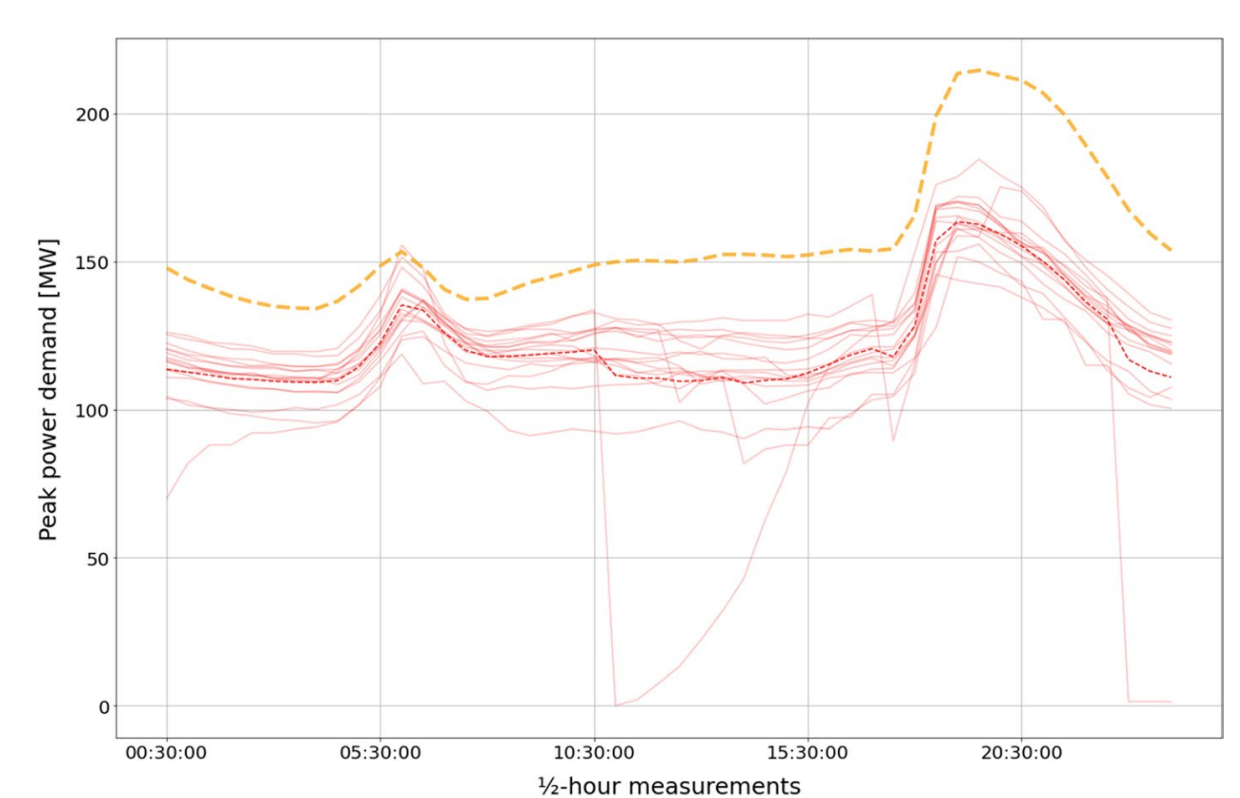
\includegraphics[width=0.6\textwidth]{figures/jessen_ndImpactedClusters/jessen_ClusterTwo2018.png}
    \caption{This figure takes a closer look at the red cluster of the earthquake-impacted year of 2018.
    The Red Solid Lines represent the Clusters' Daily Profiles, the Red dashed Line is the Average for the Red Cluster, and the thick Orange dashed Line is the daily Average for the whole 2018
    It is detectable, that the identified profiles are far from the average daily load profile of the whole year.
    The severe electricity consumption reductions happened as a result of a 7.0 Richter Scale earthquake on the northern part of Lombok on 5 August 2018.
    During the earthquake, the electricity load reduced by 78\% compared to the pre-earthquake consumption.
    The electricity system did not fully recover within a 10-day range.
    }
    \label{fig:clustering_results_2018_cluster_two}
\end{figure}

\section{Improving the Design of Energy-Saving Incentives}
\label{sec:improving_the_design_of_energy_saving_incentives}
The k-means algorithm is used in two different contexts, namely the industry and private housing sectors.
Each paragraph shows the findings of the respective sector.
\subsection{Industry}
Applying k-means with a fixed value of $k=3$, the datasets are separated into low-, mid-, and highly-efficient industry sectors or companies within these sectors.
Therefore, general patterns are detected and compared.
Spotting these general characteristics' thresholds and characteristic metrics are determined.

A clustering example of the environmental impact measured on $SO_2$ emissions is shown in Table \ref{tab:multi_industries_clustering_results_based_on_the_so2_emission}.
General high-consuming, low-efficient industry sectors are spotted, in this case for example the black metal smelting industry.
Most industry sectors remain in one cluster, a good example is the textile or rubber/plastic products industry.
Some industry sectors are represented in several clusters with a clear tendency towards one cluster, for example, the black metal smelting industry or the electricity and heat industry.
This can imply, that some companies within the industry sector are less efficient than others.
It therefore is possible for these companies not to be spotted as outliers.
The last pattern is a clear preference for a certain cluster with a few companies being represented in another cluster, for example, the paper products industry.
These companies can be spotted as outliers.
This shows, that k-means can be used to identify general cluster structures and to compare companies within industry sectors.
The detection, therefore, is a starting point for putting energy-saving incentives into action.

K-means provides the functionality to compare companies within and between industry sectors.
This is a starting point for putting energy-saving incentives into action.
Outliers in sectors can be spotted and addressed.
Therefore, applying k-means to the given dataset helps in finding a starting point in industry sectors and distinct companies for designing and applying energy-saving incentives.

\begin{table}[h]
    \centering
    \begin{tabular}{|c|c|c|c|c|}
        \hline
        \textbf{Fields} & \textbf{Sum} & \textbf{Cluster 0} & \textbf{Cluster 1} & \textbf{Cluster 2} \\
        \hline
        Chemical Industry & 144 & 138 & 0 & 6 \\
        Coal Mining and Washing Industry & 60 & 54 & 4 & 2 \\
        Black Metal Smelting & 75 & 53 & 6 & 16 \\
        Textile Industry & 49 & 49 & 0 & 0 \\
        Rubber / Plastic Products Industry & 11 & 11 & 0 & 0 \\
        Paper Products Industry & 47 & 42 & 0 & 5 \\
        Electricity, Heat Industry & 384 & 274 & 18 & 92 \\
        \hline
    \end{tabular}
    \caption{This table shows a snippet of the clustering results on all industry sectors based on the $SO_2$ emissions.
    Each industry sector is represented by a row, the columns represent the clusters showing the number of companies in each cluster.
    $k$ is fixed at $3$ since the research wants to identify low-, mid-, and high-efficient industry sectors.
    }
    \label{tab:multi_industries_clustering_results_based_on_the_so2_emission}
\end{table}

\subsection{Private Housing}
K-means is used in different contexts with different interpretations.
Malatesta et al. \cite{MAL-HBP} use k-means to identify home systems of best practices (HSOPs) in private housing.

To get an overview of the general structure of consumption patterns, the average daily energy profile of all monitored households (Figure \ref{fig:total_data_averaging}) is generated by averaging the total dataset.
The dual peak model with a dip midday proved to be the dominant HSOP of the living lab.
This provides a baseline for home comparison in the next steps.

Applying k-means clustering to the whole dataset of monitored households resulted in the clustering results shown in Figure \ref{fig:clustering_whole_dataset}.
$k=8$ was found to be the optimal number of clusters.
This depicts a more granular view of the dominant routines and habits compared to the averaged daily energy profile.
The results show, that HSOPs can be socially shared between different households, revealing dominant routines and rhythms the occupants follow.
Each cluster highlights a typical HSOP of the precinct as a whole.
Since each daily pattern is assigned to a cluster, assumptions for weekdays, weekends, holidays and seasons can be made. 
This reveals that HSOPs are different for the summer and winter seasons due to heating and cooling practices.
Also, most of the profiles show a similar dual peak pattern as the averaged profile, with peaks changing in daytime, shape and magnitude.
This shows that k-means can identify dominant HSOPs by the given data that can be used as input for higher-level social theory models that could not have been used without the k-means results.

Clustering each household separately revealed different numbers of clusters per household.
The clustering results were then complemented by a survey of the residents.
This gave insights into how different behaviors or more general traits affect the energy consumption of households.
This shows that lifestyles with different work commitments (e.g. working from home) or family structures (e.g. having children) alter the energy consumption of households \cite{KUR-HBP}.
Figure \ref{fig:routinized_household} shows a very routinized household with only two clusters.
The survey of the household's residents shows that the occupants are less flexible due to their work commitments and family structures.
This shows that repetitive structures in the daily routines of the occupants are visible in the energy consumption.
Also, k-means can spot these repetitive structures in the data which can be used complementary to the survey results.

More flexible lifestyles like working or studying from home resulted in different peaks of alternating magnitude and shape during the day.
This results in a higher number of clusters, resulting in a less routinized household with up to nine clusters.
Figure \ref{fig:non_routinized_household} represents an unroutinized household.
The varying patterns with different peaks and shapes can be explained by the results of the survey, with the residents being two adults between 40-59 years of age and a third person between 18-24 years of age.
One of the adults is working from home, the other is working away.
The third person is a student studying from home.
Since studying and working from home is not observed with typical work patterns, the energy consumption is more flexible explaining the different times of the peaks.
This shows that changes in behaviors most likely result in a change in energy consumption.
This finding is supported by the second result, that if occupants are routinized, their behaviors are repetitive \cite{BRE-EWP}.

K-means proved that repetitive structures in the daily routines of the occupants are visible in the energy consumption.
Also, changes in behavior result in a change in energy consumption.
This shows that k-means can be successfully applied in this context, and serve as input for higher-level social theory models that could not have been used without the k-means results.

\begin{figure}
    \centering
    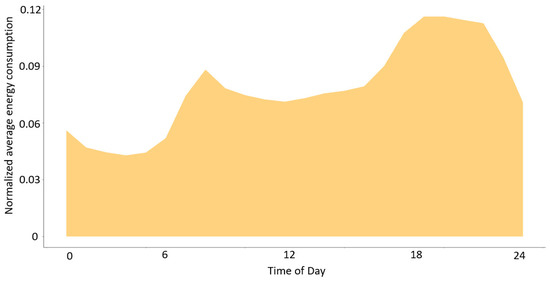
\includegraphics[width=0.6\textwidth]{figures/malatesta_hsop/malatesta_totalDataAveraging.jpg}
    \caption{This graph shows the average daily energy profile from all monitored homes.
    This provides a baseline for individual home comparison.
    It demonstrates the general consumption pattern for the households.
    A dual peak model with a dip midday is the average consumption habit.
    }
    \label{fig:total_data_averaging}
\end{figure}

\begin{figure}
    \centering
    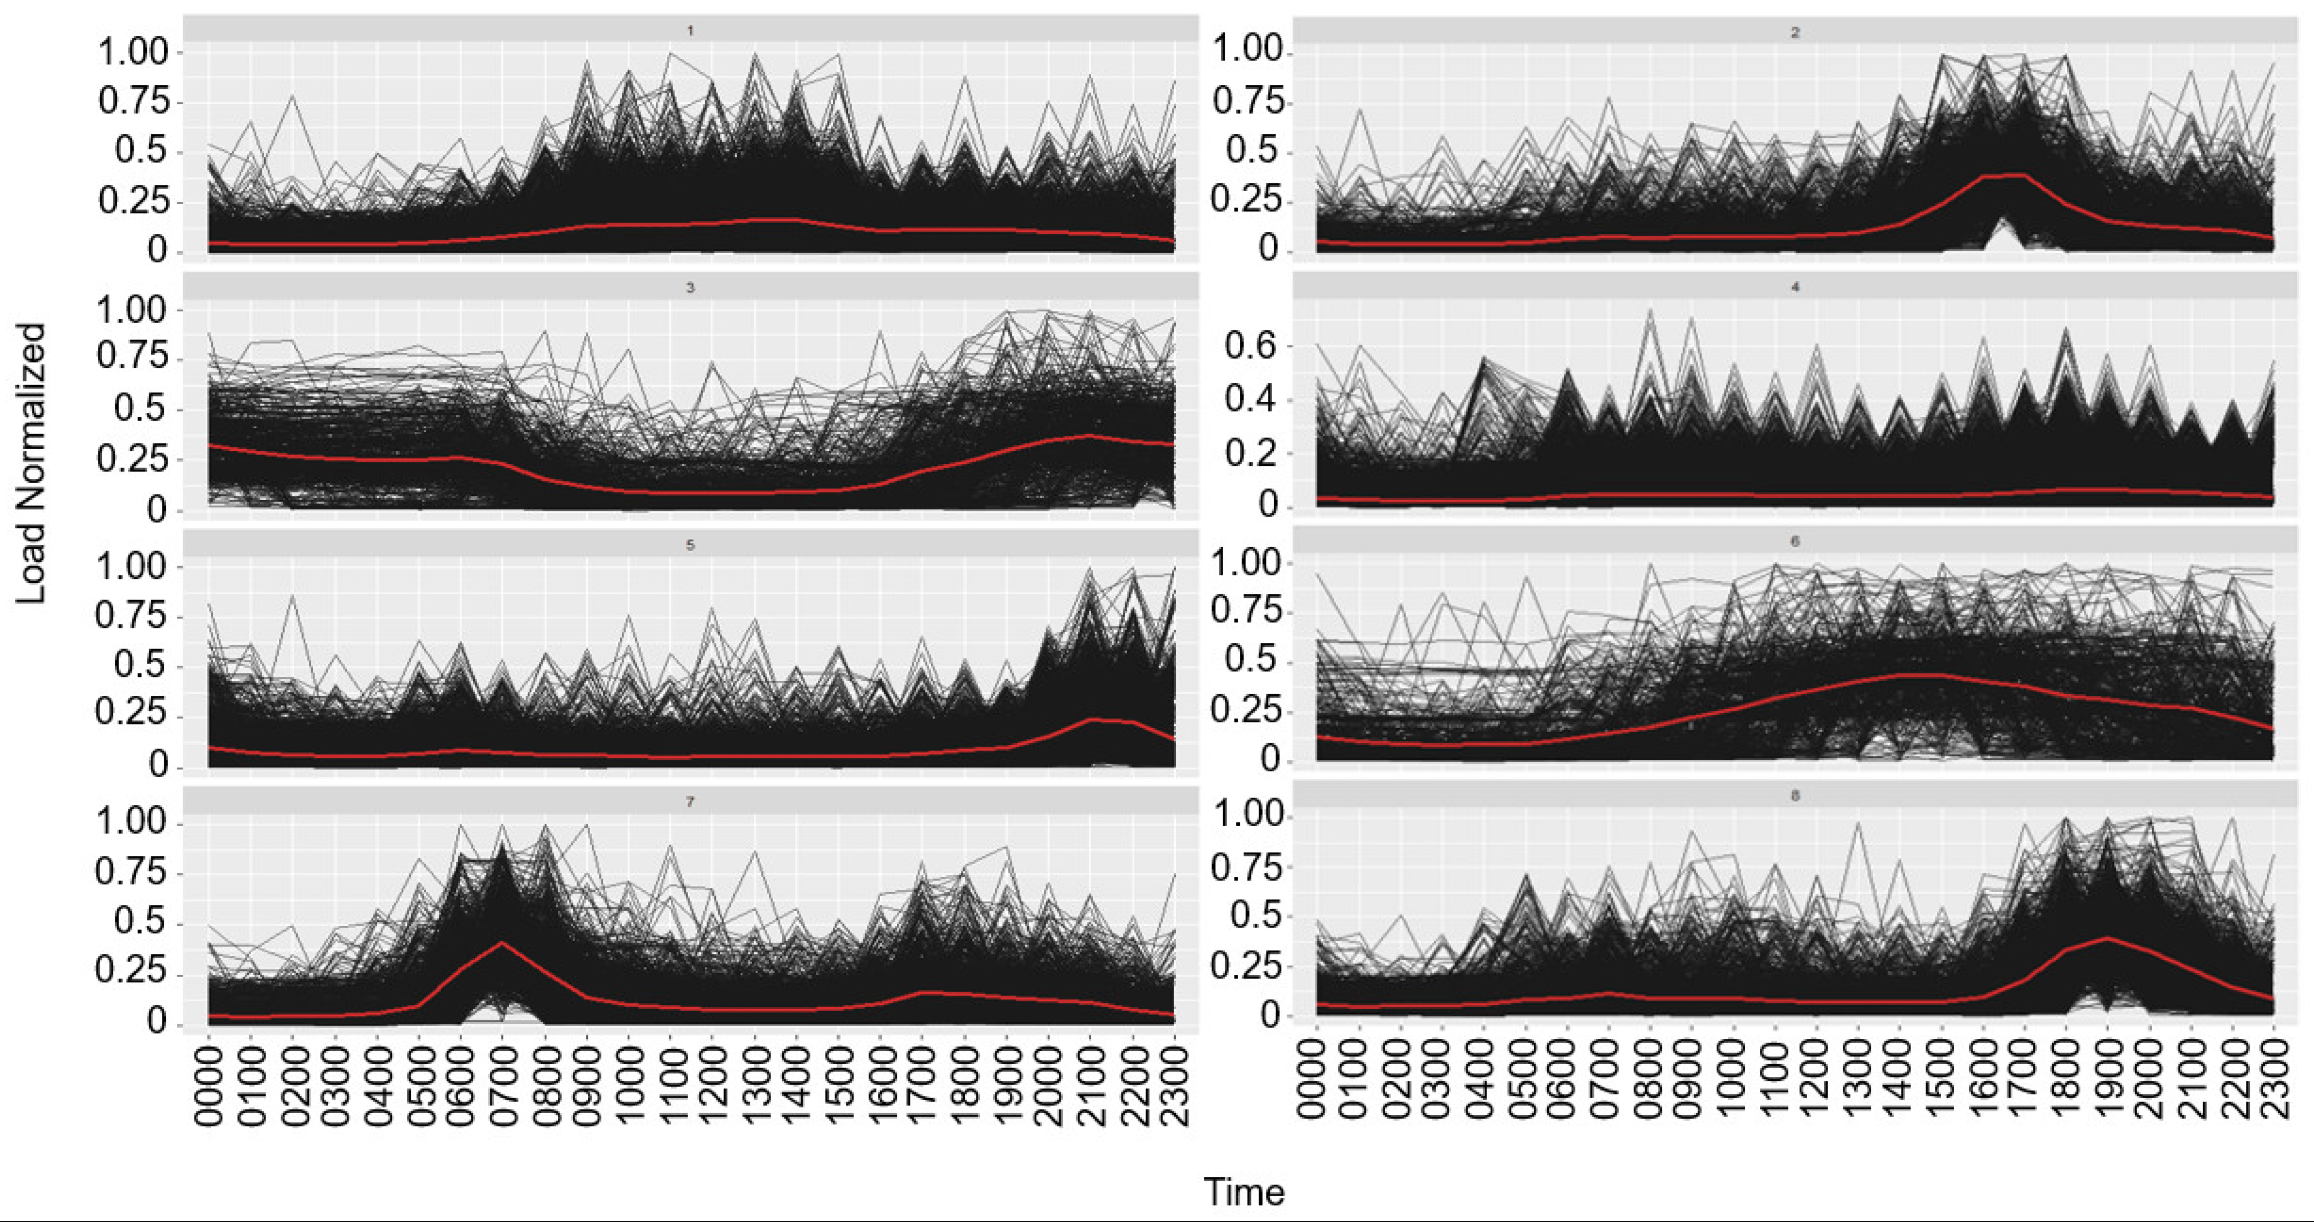
\includegraphics[width=0.7\textwidth]{figures/malatesta_hsop/malatesta_clusteringWholeDataset.png}
    \caption{These clusters are the result of clustering the whole dataset of monitored households.
    Each cluster represents a dominant HSOP, with the red line representing the average consumption in the cluster and the black lines the assigned daily profiles.
    However, more than half of the profiles show a similar dual peak pattern with a dip midday.
    Seasonal patterns are visible, with cluster 7 being a summer pattern with increased energy consumption during midday and cluster 2 being a winter pattern with increased energy consumption in the morning and evening.
    }
    \label{fig:clustering_whole_dataset}
\end{figure}

\begin{figure}
    \centering
    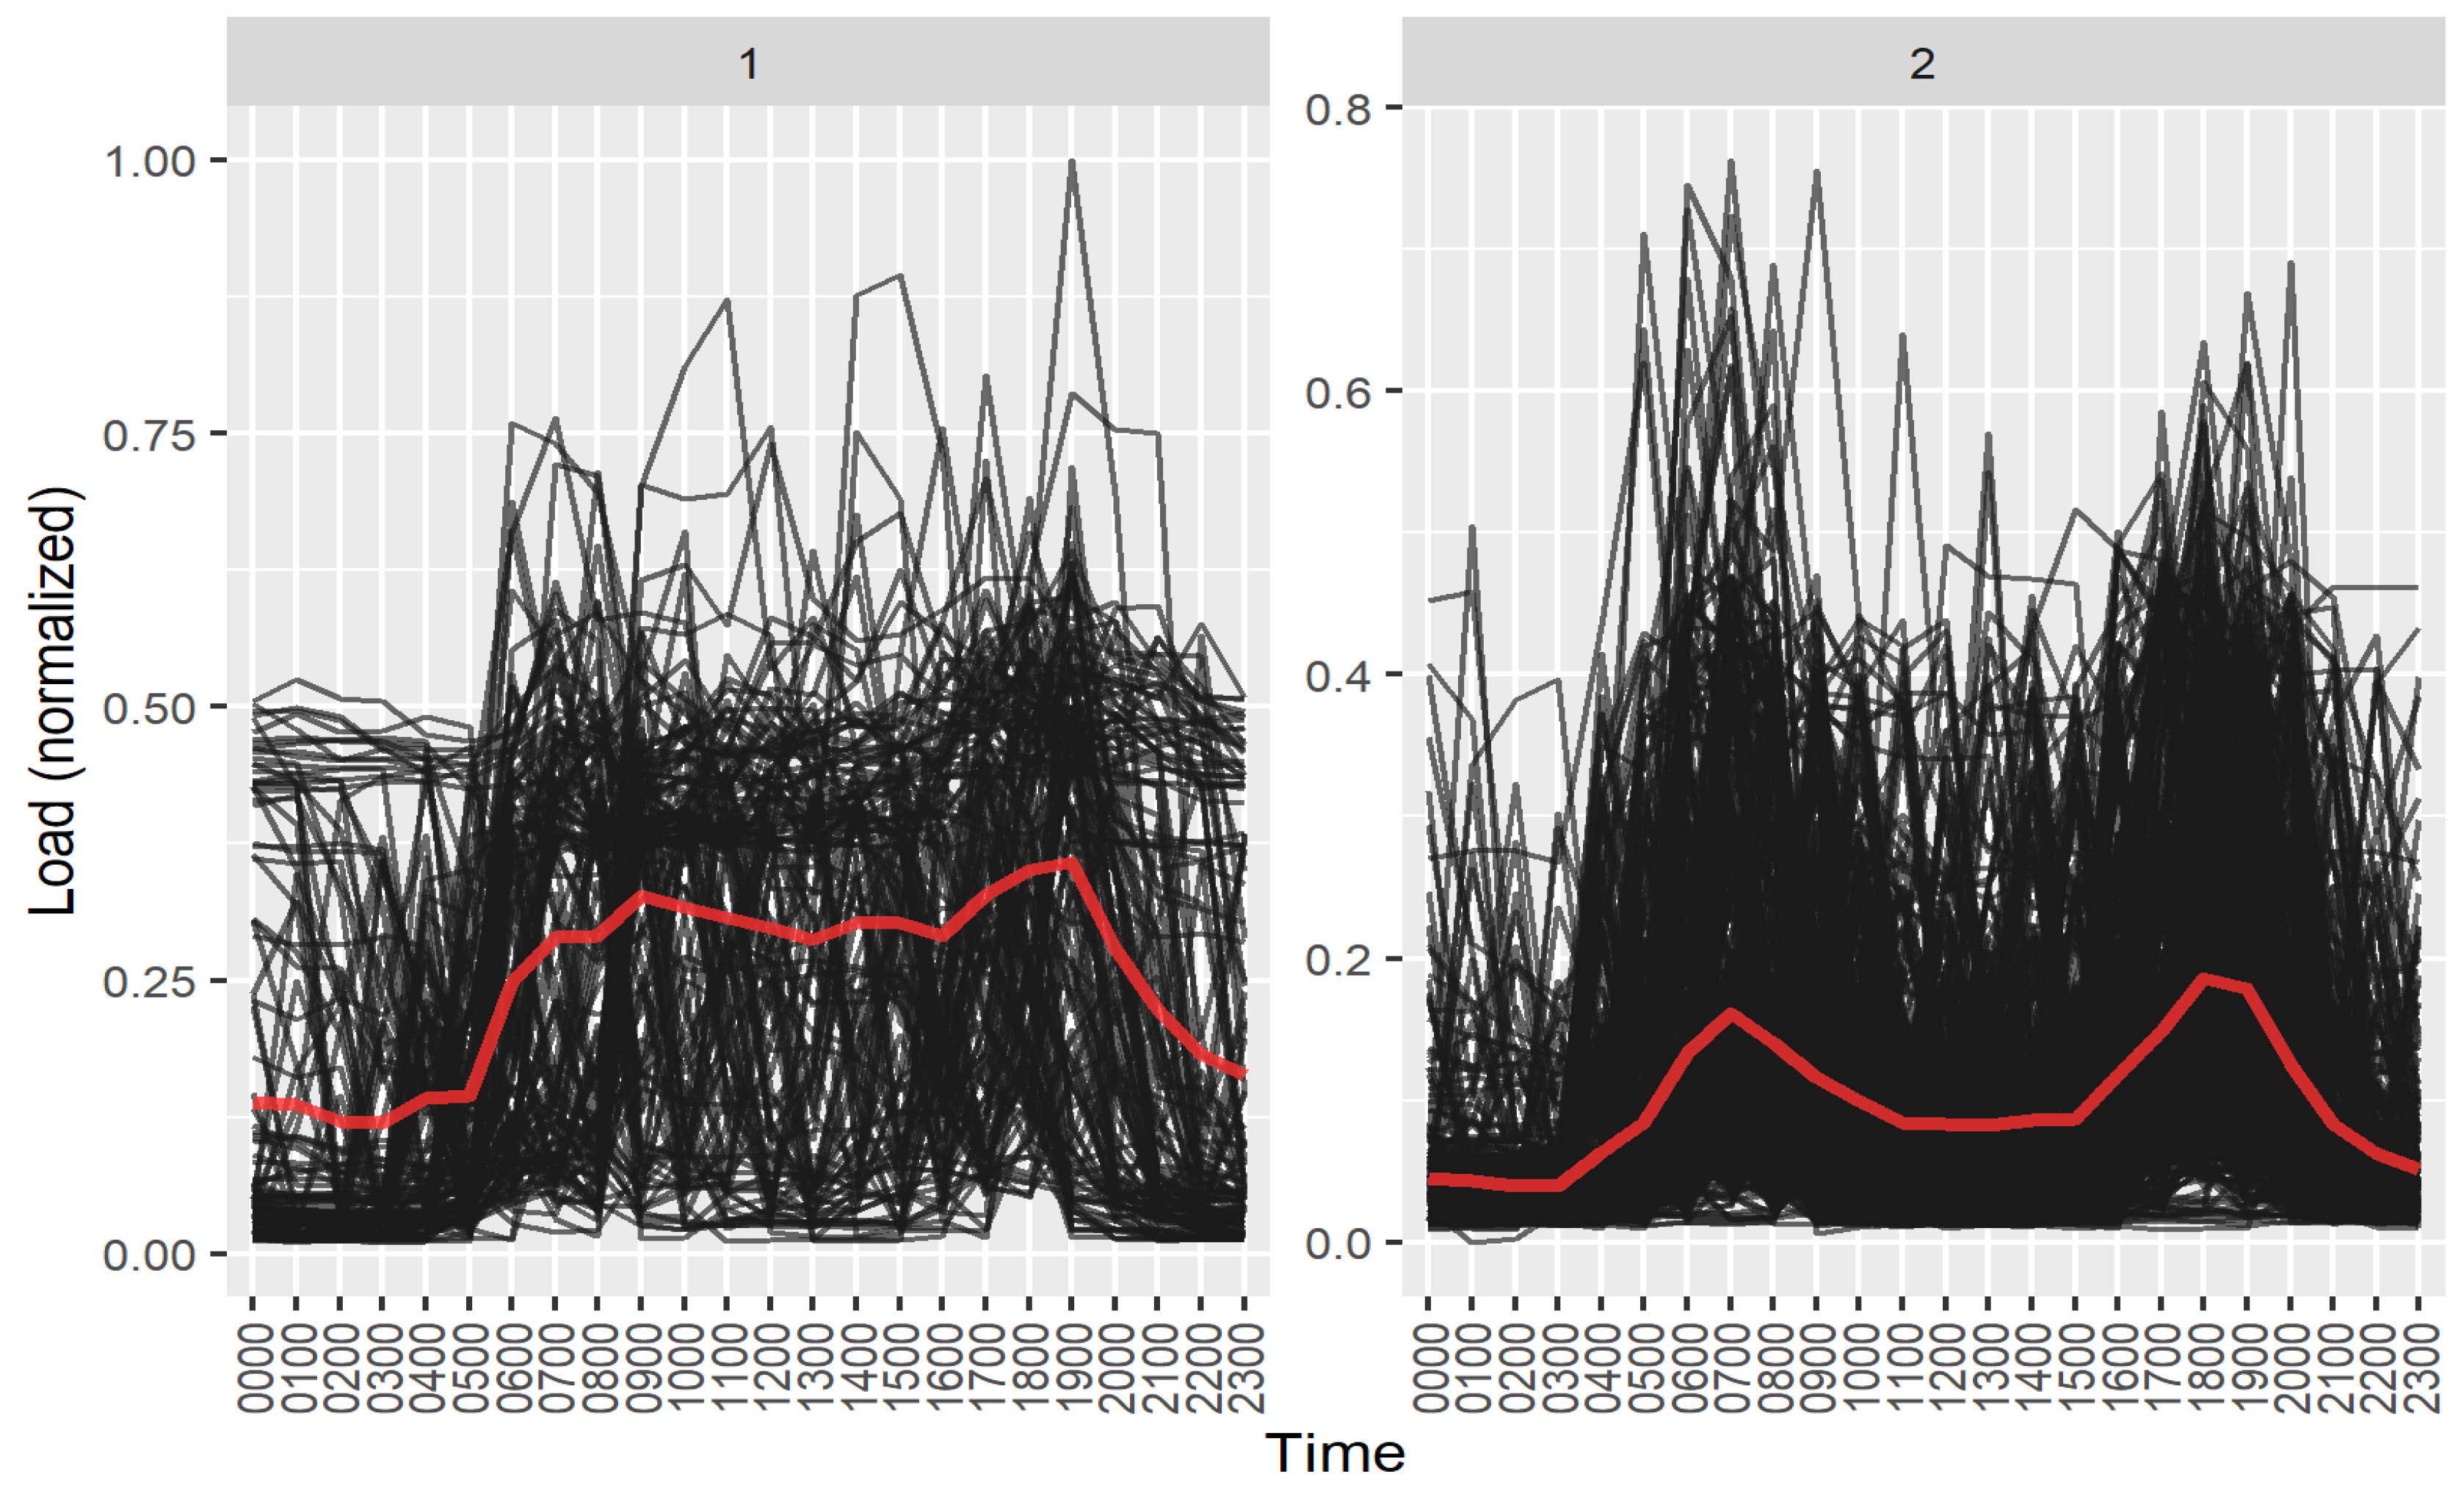
\includegraphics[width=0.6\textwidth]{figures/malatesta_hsop/malatesta_routinisedHousehold.jpg}
    \caption{These graphs represent a very routinized household with only two clusters.
    The left profile shows a broad peak during the day, it occurred mostly on weekends.
    The right profile shows a dual peak pattern with a dip midday, occurring mostly on weekdays.
    These results can be explained by the residents' working commitments and family structures making them less flexible, more repetitive, and therefore routinized.
    }
    \label{fig:routinized_household}
\end{figure}

\begin{figure}
    \centering
    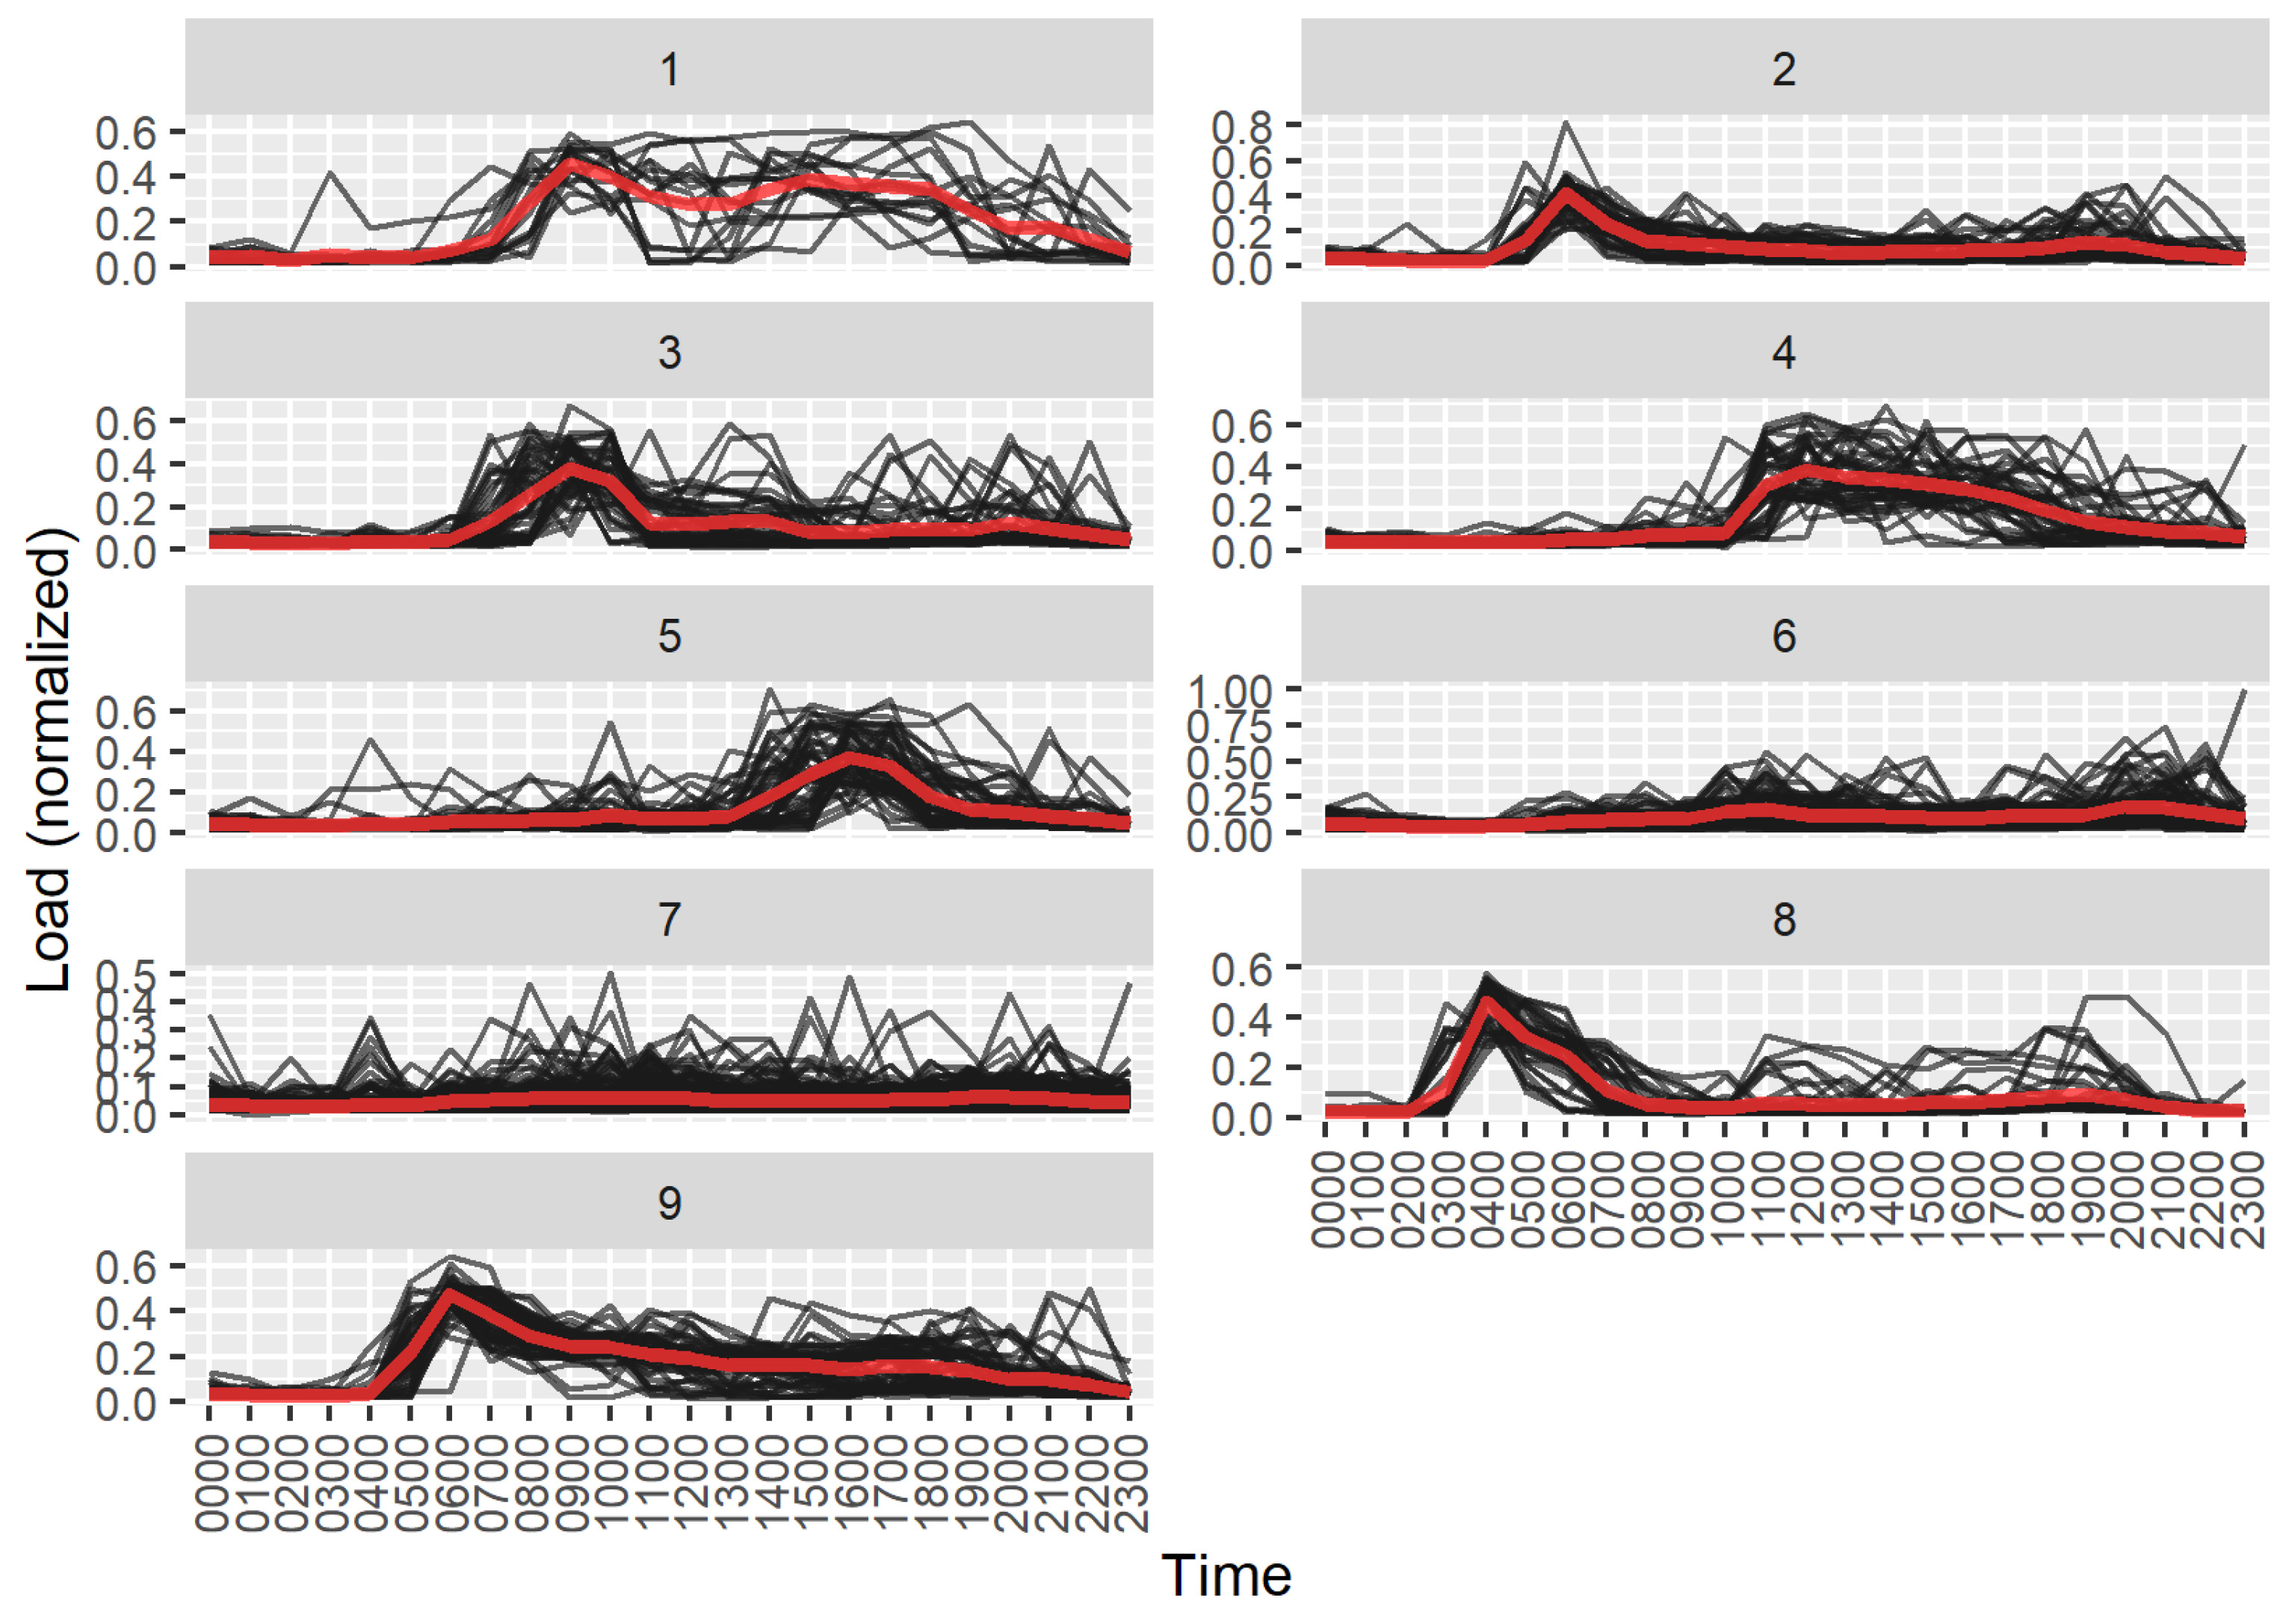
\includegraphics[width=0.6\textwidth]{figures/malatesta_hsop/malatesta_unroutinisedHousehold.jpg}
    \caption{This graph shows the other extreme with nine clusters.
    This household is less routinized than the previous one.
    The time in which the peak occurs differs between all of the nine clusters.
    They also differ in their shape and magnitude.
    These results can be explained due to the residents working and studying from home making them more flexible and less repetitive in their daily routines.
    }
    \label{fig:non_routinized_household}
\end{figure}




